\documentclass[10pt,usepdftitle=false]{beamer}

\usepackage[american]{babel}
\usepackage[utf8]{inputenc}
%\usepackage{soul}
%\usepackage{amsmath}
%\usepackage{amssymb}
\usepackage{textcomp}
\usepackage{listings}
\lstset{
  language=haskell,
  upquote=true,
  basicstyle=\ttfamily,          % print whole listing in typewriter
  keywordstyle=\color{blue}\bfseries, % bold blue keywords
  %identifierstyle=,           % nothing happens
  commentstyle=\color{green}, % green comments
  stringstyle=\color{red},      % typewriter type for strings
  showstringspaces=false     % no special string spaces
}
\usepackage[all]{xy}
\usepackage{tikz}
\usetikzlibrary{arrows,shapes,automata}
\usepackage{graphicx}
\usepackage[bibstyle=beamer,citestyle=authoryear-comp,doi=false,isbn=false,eprint=false,maxnames=10]{biblatex}
\bibliography{../defeo}
\usepackage{../mysymbols}
\usepackage{array}

\mode<presentation>{%
  \usetheme{these}
}

\title[Fast Algorithms for Towers of Finite Fields and Isogenies]{
  \def\svgwidth{2.63ex}
  \def\exclfont{\scriptsize\rmfamily}
  %% Creator: Inkscape inkscape 0.48.0, www.inkscape.org
%% PDF/EPS/PS + LaTeX output extension by Johan Engelen, 2010
%% Accompanies image file 'bigescargot-color.pdf' (pdf, eps, ps)
%%
%% To include the image in your LaTeX document, write
%%   \input{<filename>.pdf_tex}
%%  instead of
%%   \includegraphics{<filename>.pdf}
%% To scale the image, write
%%   \def\svgwidth{<desired width>}
%%   \input{<filename>.pdf_tex}
%%  instead of
%%   \includegraphics[width=<desired width>]{<filename>.pdf}
%%
%% Images with a different path to the parent latex file can
%% be accessed with the `import' package (which may need to be
%% installed) using
%%   \usepackage{import}
%% in the preamble, and then including the image with
%%   \import{<path to file>}{<filename>.pdf_tex}
%% Alternatively, one can specify
%%   \graphicspath{{<path to file>/}}
%% 
%% For more information, please see info/svg-inkscape on CTAN:
%%   http://tug.ctan.org/tex-archive/info/svg-inkscape

\begingroup
  \makeatletter
  \providecommand\color[2][]{%
    \errmessage{(Inkscape) Color is used for the text in Inkscape, but the package 'color.sty' is not loaded}
    \renewcommand\color[2][]{}%
  }
  \providecommand\transparent[1]{%
    \errmessage{(Inkscape) Transparency is used (non-zero) for the text in Inkscape, but the package 'transparent.sty' is not loaded}
    \renewcommand\transparent[1]{}%
  }
  \providecommand\rotatebox[2]{#2}
  \ifx\svgwidth\undefined
    \setlength{\unitlength}{153.08584512pt}
  \else
    \setlength{\unitlength}{\svgwidth}
  \fi
  \global\let\svgwidth\undefined
  \makeatother
  \begin{picture}(1,0.63533296)%
    \put(0,0){\includegraphics[width=\unitlength]{\artdir/bigescargot\suffix.pdf}}%
    \put(0.94506612,0.46275528){\color[rgb]{0,0,0}\makebox(0,0)[lb]{\smash{\exclfont\textbf{!}}}}%
  \end{picture}%
\endgroup
~~~Fast Algorithms\\
  \normalsize\textcolor{black}{for Towers of Finite Fields\\and Isogenies}}
\hypersetup{pdftitle={Fast Algorithms for Towers of Finite Fields and Isogenies},pdfauthor={Luca De Feo}}
\author{Luca~De~Feo}
\institute[LIX \& INRIA Saclay]{LIX, École Polytechnique \& INRIA Saclay, Projet TANC}
\date[December 13, 2010]{December 13, 2010\\École Polytechnique, Palaiseau}


\AtBeginSection[]
{
  \begin{frame}<beamer>
    \frametitle{Outline}
    \tableofcontents[currentsection]
  \end{frame}
}


\begin{document}

{\setbeamertemplate{footline}[default]
\begin{frame}
  \frametitle{PhD 2.0}
  
  \begin{center}
    \Large Connect to the WiFi network\footnote{This WiFi does not
      give you access to the WWW (not even DNS, sorry for
      IP-over-DNSers)}\footnote{No
      DOSes, please.}:\\
    \emph{\textbf{Luca's defense}} \end{center}

  \bigskip

  Open your browser, navigate to any page, and experience free
  access to:
  \begin{itemize}
  \item electronic manuscript,
  \item electronic presentation, %(in three languages),
  \item live cast of the defense,
  \item many other goodies!
  \end{itemize}

  \bigskip

  Also check us out on: \emph{\url{http://crypto.lix.polytechnique.fr/}}
\end{frame}
}

%%

{\setbeamertemplate{footline}[these theme title]
\begin{frame}
  \titlepage
\end{frame}
}

%%
%%

\setcounter{framenumber}{0}
\section{Introduction}

\begin{frame}
  \frametitle{The Discrete Logarithm Problem}
  
  \begin{columns}
    \begin{column}{0.4\textwidth}
      \begin{tikzpicture}
        \begin{scope}
          \foreach \alpha in {0,...,4} {
            \filldraw (-65-25*\alpha:2) circle (2pt);
          }
          \foreach \alpha in {0,...,3} {
            \draw[->] (-65-25*\alpha:2) arc (-65-25*\alpha:-85-25*\alpha:2);
            \draw (-90-25*\alpha:2.3) node {$g^\alpha$};
          }
          \draw (-65:2.3) node {$g^{n-1}$};
          \draw[densely dotted,gray] (-65:2) arc (-65:195:2);
          \draw (0,0) node {\Large $G=\langle g\rangle$};
        \end{scope}
        
        \begin{uncoverenv}<2->
          \begin{scope}[yshift=-3cm]
            \foreach \alpha in {0,...,4} {
              \filldraw (-65-25*\alpha:2) circle (2pt);
            }
            \foreach \alpha in {0,...,3} {
              \draw[->] (-65-25*\alpha:2) arc (-65-25*\alpha:-85-25*\alpha:2);
              \draw (-90-25*\alpha:2.3) node {$\alpha$};
            }
            \draw (-65:2.3) node {$n-1$};
            \draw[densely dotted,gray] (-65:2) arc (-65:48:2);
            \draw[densely dotted,gray] (132:2) arc (132:195:2);
            \draw (0,-0.5) node {\Large $\Z/n\Z$};
          \end{scope}
        \end{uncoverenv}
        
        \begin{uncoverenv}<3->
          \foreach \alpha in {0,...,4}
          \usebeamercolor[fg]{alerted text}
          \draw[dashed] (-65-25*\alpha:2) -- ++(0,-3cm);
        \end{uncoverenv}
      \end{tikzpicture}
    \end{column}
    \begin{column}{0.6\textwidth}
      \begin{block}{Exponentiation in a cyclic group}
        Let $G=\langle g\rangle$ be a cyclic group of order $n$.
        Define
        \begin{align*}
          \exp_g : \Z/n\Z &\ra G\text{,}\\
          x&\mapsto g^x\text{.}
        \end{align*}
      \end{block}

      \begin{block}<2->{Discrete logarithm} $\exp_g$ is an
        isomorphism. Its inverse is called \emph{discrete logarithm}.
        \begin{align*}
          \log_g : G &\ra \Z/n\Z\text{,}\\
          g^x&\mapsto x\text{.}
        \end{align*}

        \begin{uncoverenv}<3-> Computing it is called the
          \alert{Discrete Logarithm Problem} (DLP) of $G$.
        \end{uncoverenv}
      \end{block}
    \end{column}
  \end{columns}
\end{frame}

%%

\begin{frame}
  \frametitle{Elliptic curve cryptography}

  \vspace{-1mm}

  \begin{columns}
    \begin{column}{0.4\textwidth}
      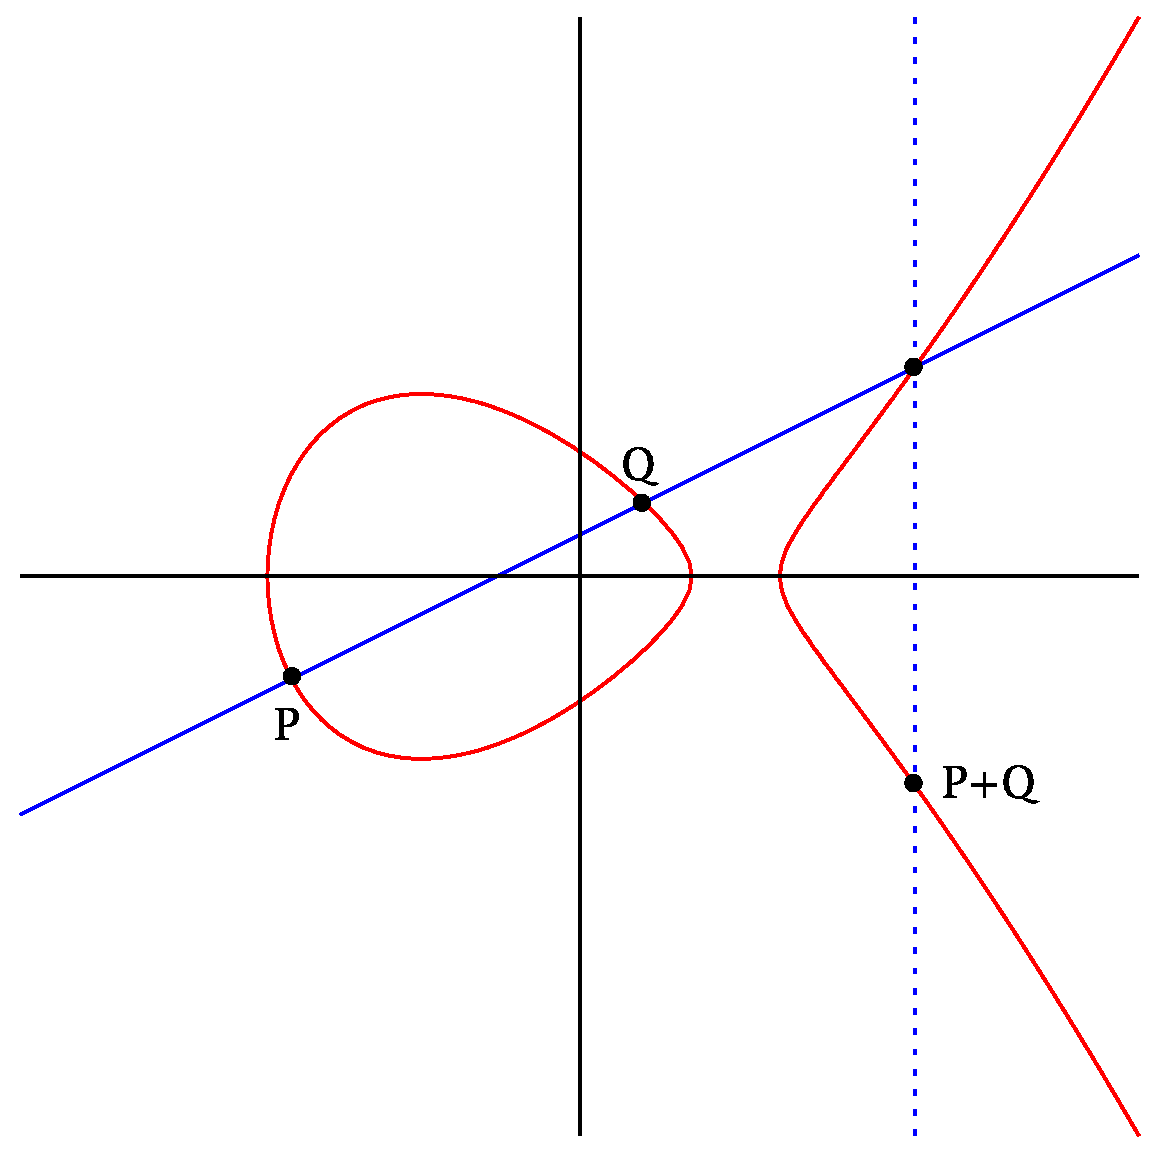
\includegraphics[width=\textwidth]{../isogeny/ec-add.pdf}
    \end{column}
    \begin{column}{0.55\textwidth}
      \begin{block}{Elliptic curve (Weierstrass form)}
        \[E : y^2 = x^3 + ax + b\text{;}\]
      
        The set of points of an elliptic curve is endowed with a group
        law via the chord-and-tangent law.
      \end{block}
    
      \begin{block}{}
        \emph{Hasse bound:} $\card{E(\F_q)} \sim q$.
      \end{block}
    \end{column}
  \end{columns}

  \begin{center}
    \begin{tabular}{l | l | l}
      &\emph{\textbf{Finite field crypto}} & \emph{\textbf{Elliptic curve crypto}}\\
      \hline
      \emph{Group} & $\F_q^\ast$ & $E(\F_q)$\\
      \emph{Protocols} & El Gamal, DSA, \dots & ECDH, ECDSA, ECMQV, \dots\\
      \emph{Key sizes} & 1024, 2048, 3072 & 160, 225, 256 \\
    \end{tabular}
  \end{center}

\end{frame}

%%

\begin{frame}
  \frametitle{Group law and scalar multiplication}
  
  \begin{columns}
    \begin{column}{0.3\textwidth}
      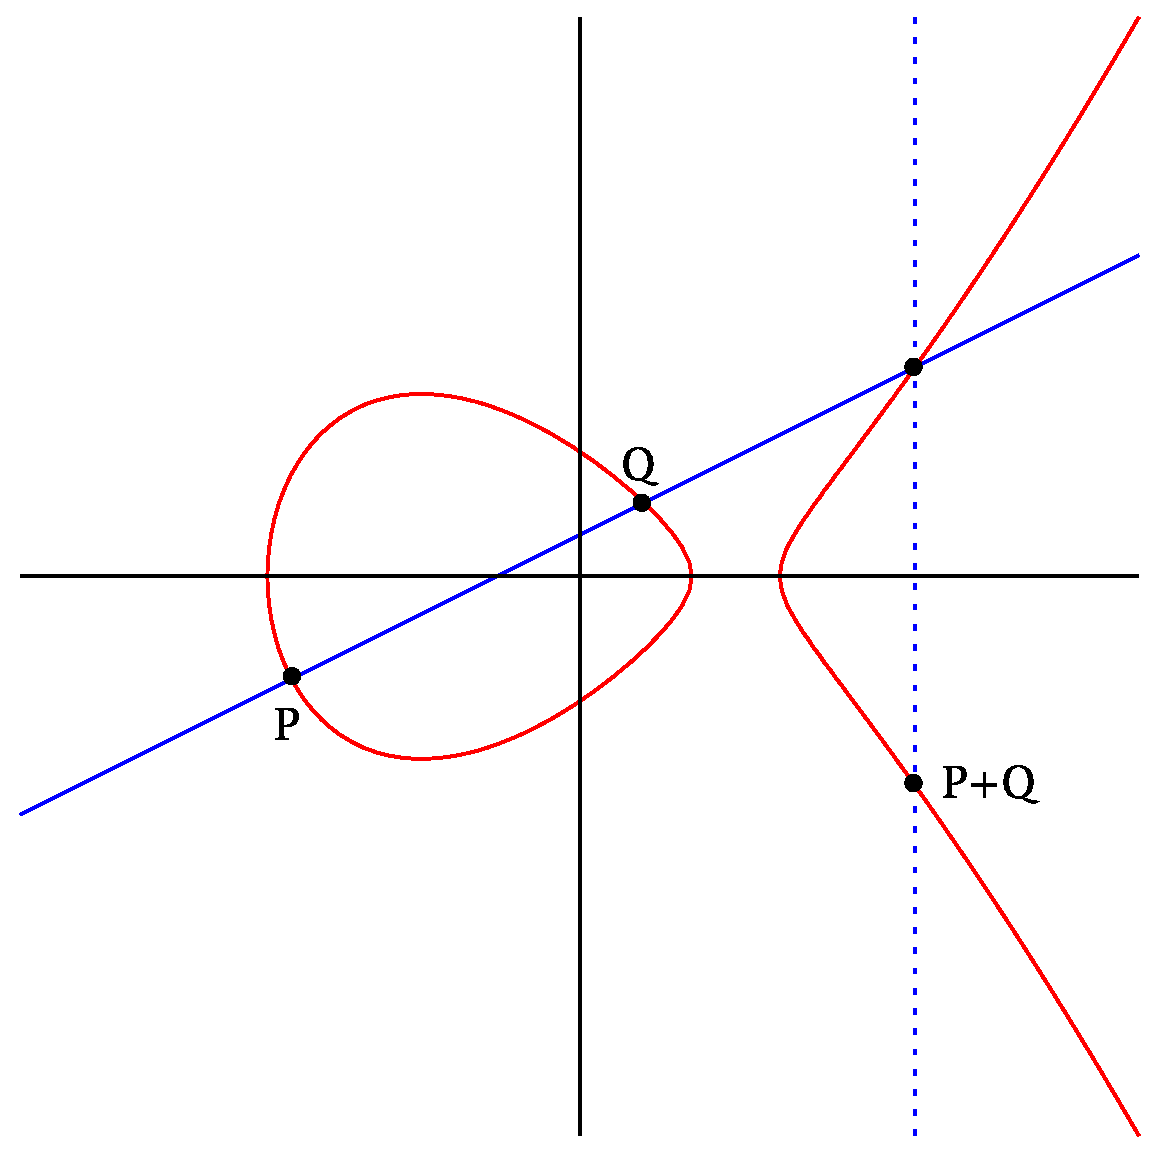
\includegraphics[width=\textwidth]{../isogeny/ec-add.pdf}
    \end{column}
    \begin{column}{0.55\textwidth}
      {\large\emph{\[y^2 = x^3 + ax + b\]}}
      \begin{gather*}
        P = (x_0, y_0), Q = (x_1, y_1)\\
        \lambda = \frac{y_1 - y_0}{x_1 - x_0}\\
        P+Q = (\lambda^2 - x_0 - x_1, (x_0 - x_2)\lambda - y_0)
      \end{gather*}
    \end{column}
  \end{columns}

  {\large
    \begin{description}
    \item[\emph{Multiplication:}] $[m]P = \overbrace{P + P + \cdots + P}^{\text{$m$ times}}$
    \item[\emph{$m$-torsion:}] $E[m] = \{P\in E(\clot{\K}) | [m]P=\0\} \isom (\Z/m\Z)^2$
    \end{description}}
  
  \[[m](x,y) = \left(\frac{\psi_m(x,y)}{\phi_m^2(x,y)}, \frac{\omega_m(x,y)}{\phi_m^3(x,y)}\right)\]
  
  \emph{Division polynomials:} $\phi_m$ can be computed with $O(\log
  m)$ polynomial multiplications, $\deg\phi_m=O(m^2)$.
\end{frame}

%%

\begin{frame}
  \frametitle{Isogenies between elliptic curves}
  
  \vspace{-5mm}

  {\large \[\xymatrix{E\ar[d]_{[m]}\ar[r]^{\I} & E'\ar[dl]^{\hat{\I}}\\E}\]} 
  \emph{\textbf{(Separable) isogeny:}} (separable)
  non-constant rational morphism preserving the identity.
  
  \begin{block}{Properties}
    \begin{itemize}
    \item Isogeny = rational map $\;+\;$ group morphism;
    \item Finite kernel, surjective (in $\clot{\K}$);
    \item \emph{Dual isogeny theorem:} they factor the multiplication map into two pieces.
    \end{itemize}
  \end{block}

  \vspace{-1mm}

  \begin{block}{
	\begin{overprint}
	\onslide<1> Multiplication	
	\onslide<2> Frobenius endomorphism
	\onslide<3> Separable isogeny (simplified Weierstrass model)
	\end{overprint}
      }
    \begin{overprint}
      \onslide<1>
      \[\begin{aligned}
	{}[m] : E(\clot{\K}) &\rightarrow E(\clot{\K})\\
	                   P &\mapsto [m]P
      \end{aligned}\]
      $\ker\I = E[m]$.

      \onslide<2>
      \[\begin{aligned}
	\frob : E(\clot{\K}) &\rightarrow E(\clot{\K})\\
	               (x,y) &\mapsto (x^q,y^q)
      \end{aligned}\]
      $\ker\frob = \{\0\}$.

      \onslide<3>
      \[\quad\I(x,y) = \left(\frac{g(x)}{h(x)},
      cy\left(\frac{g(x)}{h(x)}\right)'\right)\]
      $h\;$ vanishes on the abscissas of $\;\ker\I$. \emph{$\quad\deg\I \;=\; \card{\ker\I}$}.
    \end{overprint}
  \end{block}  
\end{frame}

%%

\begin{frame}
  \frametitle{Why compute (large) isogenies over finite fields?}
  
  \begin{block}{SEA algorithm (\cite{schoof85,elkies92,atkin88})}
    \begin{description}
    \item[Hasse bound] \hfill{\large\emph{$\card{E(\F_q)}= q-t+1$}};\hfill\strut
    \item[Schoof] Compute $t$ modulo small primes
      $\ell\;\Leftrightarrow$ compute the action of $\frob_q$ on
      \emph{$E[\ell]\;\isom\;(\Z/\ell\Z)^2$};
    \item[Atkin] Determine the order of the roots of $X^2 -tX +q$ by
      factoring the $\ell$-th modular polynomial.
    \item[Elkies] Compute an $\ell$-isogeny $\I$ and the action of
      $\frob_q$ on \emph{$\ker\I\;\isom\;\Z/\ell\Z\;\subset\;E[\ell]$};
    \end{description}
  \end{block}

  \begin{block}{Other cryptographic applications}
    \begin{itemize}
    \item Transfer DLPs between curves (\cite{gaudry+hess+smart02,smith09});
    \item Construct new cryptosystems (\cite{teske06,rostovtsev+stolbunov06});
    \item Construct hash functions (\cite{charles+lauter+goren09});
    \item Compute modular polynomials (\cite{sutherland10:modpol});
    \item Compute the endomorphism ring (\cite{kohel,sutherland10:hilbert}).
    \end{itemize}
  \end{block}
\end{frame}

%%
%%

\section{Computing isogenies over finite fields}

\begin{frame}
  \frametitle{Vélu's formulas}
  
  \begin{block}{Compute an isogeny with given kernel (\cite{velu71})}
    Given the kernel $H$, computes $\;\I : E\to E/H\;$ given by
    \begin{align*}
      &\I(\0_E) = \I(\0_{E/H})\text{,}\\
      &\begin{aligned}
        \I(P) = \Biggl(x(P) + \sum_{Q\in H^\ast}x(P+Q) - x(Q),
        y(P) + \sum_{Q\in H^\ast}y(P+Q) - y(Q) \Biggr) \text{.}
      \end{aligned}
    \end{align*}
  \end{block}

  \begin{block}{In practice, given $h(x)$ vanishing on $H$}
    {\footnotesize
      \[
      y^2 = f(x)
      \qquad
      t = \sum_{Q\in H^\ast} f'(Q)\text{,}
      \quad
      u = \sum_{Q\in H^\ast} 2f(Q)\text{,}
      \quad
      w = u + \sum_{Q\in H^\ast} x(Q)f'(Q)\text{,}\]}
    \[\alert{\I(x,y) = \left(\frac{g(x)}{h(x)}, y\left(\frac{g(x)}{h(x)}\right)'\right)}
    \quad\text{with}\quad
    \frac{g(x)}{h(x)} = x + t\frac{h'(x)}{h(x)} - u\left(\frac{h'(x)}{h(x)}\right)'\]
  \end{block}
\end{frame}

%%

\begin{frame}
  \frametitle{Isogeny computation}
  By Vélu's formulas: $\I(x,y) = \left(\frac{g(x)}{h(x)},
    y\left(\frac{g(x)}{h(x)}\right)'\right)$, hence
  \[(x^3 + ax + b){\left(\frac{g(x)}{h(x)}\right)'}^2 =
  \left(\frac{g(x)}{h(x)}\right)^3 + a'\frac{g(x)}{h(x)} + b'\]
  
  \begin{block}{\textbf{Algorithms:} Given $E, E', \ell$, compute $\I:E\to E'$}
    \begin{itemize}
    \item \emph{\cite{strak73}}: First algorithm in characteristic
      $0$, using continued fractions.
    \item \emph{\cite{elkies92,elkies98}:} Find a power series
      solution to the differential equation.
    \item \emph{\cite{couveignes94}:} Compute morphisms of formal
      groups, look for one that corresponds to an isogeny.
    \item \emph{\cite{couveignes96}:} Interpolate over the
      $p$-torsion, look for a polynomial that corresponds to an
      isogeny.
    \item \emph{\cite{lercier96}:} (only for $p=2$) solve a linear
      system.
    \item \emph{BMSS
        algorithm \parencite{bostan+morain+salvy+schost08}:} Improve
      \cite{elkies98} to run in quasi-linear time.
    \item \emph{\cite{lercier+sirvent08}:} Lift $E$ and $E'$ in the
      $p$-adics, then apply BMSS.
    \end{itemize}
  \end{block}
\end{frame}

%%

\begin{frame}
  \frametitle{Couveignes' algorithm (\cite{couveignes96})}
  
  \begin{center}
    \large
    Given $E, E', \ell$, compute $\I:E\to E'$
  \end{center}

  \begin{center}
    \emph{\textbf{Idea:}} Send $E[p^k]$ over $E'[p^k]$
  \end{center}
  
  \begin{itemize}
  \item Compute the extensions $\U_i/\F_q$ such that $E[p^i]$ is
    defined in $\U_i$;
    \uncover<1-2>{\hfill\emph{\alt<1>{$\tildO(\ell^2)$}{\alert{$\tildO(\Mult(\ell))$}}}}
  \item Pick $\;k\;$ \emph{large enough} ($k\sim\log_p4\ell$);
  \item Compute $\;P$, a generator of $\;E[p^k]$;
    \uncover<1-2>{\hfill\emph{\alt<1>{$\tildO(\ell^2)$}{\alert{$\tildO(\Mult(\ell))$}}}}
  \item Compute $\;P'$, a generator of $\;E'[p^k]$;
    \uncover<1-2>{\hfill\emph{\alt<1>{$\tildO(\ell^2)$}{\alert{$\tildO(\Mult(\ell))$}}}}
  \item Compute the polynomial $\;T\;$ vanishing on $\;E[p^k]$;
    \uncover<1-2>{\hfill\emph{\alt<1>{$\tildO(\ell^2)$}{\alert{$\tildO(\Mult(\ell))$}}}}
  \item For $m\in\left(\Z/p^k\Z\right)^\ast$
    \begin{itemize}
      \normalsize
    \item Interpolate $\;A : x(P) \mapsto x([m]P')$;
      \uncover<1-2>{\hfill\emph{\alt<1>{$\tildO(\ell^2)$}{\alert{$\tildO(\Mult(\ell))$}}}}
    \item Reconstruct a rational fraction  $\;\frac{g}{h}\equiv A \bmod T$;
      \uncover<1-2>{\hfill\emph{$\tildO(\Mult(\ell))$}}
    \end{itemize}
    \alert<3>{Stop when $\frac{g}{h}$ is an isogeny.}
    \uncover<1-2>{\hfill\emph{$\ell$ times on average}}
  \end{itemize}
\end{frame}

%%

\begin{frame}
  \frametitle{How to recognize an isogeny?}

  \begin{itemize}
    \setlength{\itemsep}{\baselineskip}
  \item \emph{\textbf{Degree:}} $\frac{g}{h}\;$ with $\;\deg g=\ell$, $\;\deg h = \ell-1$;\hfill\alert{$O(1)$}
  \item \emph{\textbf{Square factor:}} $h = \prod_{Q\in H^\ast}(X-
    x(Q)) = f^2\;$ if $\ell$ odd;\hfill\emph{$\tildO(\Mult(\ell))$}
  \item \emph{\textbf{Group action:}} Test on random points: $\;\I(P+Q)=\I(P)+\I(Q)$;\hfill\emph{$O(\ell)$}
  \item \emph{\textbf{Factor of the $\ell$-division polynomial:}}
    Compute $\phi_\ell\bmod h$.\hfill\emph{$\tildO(\Mult(\ell))$}
  \end{itemize}
\end{frame}

%%

\begin{frame}
  \frametitle{How to recognize an isogeny?}
  
  \begin{center}
    $T\;$ vanishes on $\;E[p^k]$, $A$ interpolates $x(P)\mapsto x(P')$
  \end{center}
  
  \[AU_i + TV_i = R_i  \qquad\Leftrightarrow\qquad  A\equiv \frac{R_i}{U_i} \bmod T\]
  \[\ell = 11\]
  \pause
  \begin{center}
  \begin{tabular}{c | c}
    $\deg R_i$ & $\deg U_i$ \\
    $3141592653589793238462643$ & 0 \\
    \pause
    $3141592653589793238462642$ & 1 \\
    \pause
    $3141592653589793238462641$ & $2$ \\
    \pause
    \vdots & \vdots\\
    $3141592653589793238462634$ & $9$ \\
    \pause
    \Huge\alert{$11$} & \Huge\alert{$10$}\\
    \pause
    $10$ & $3141592653589793238462633$\\
    \vdots & \vdots
  \end{tabular}
  \end{center}
\end{frame}

%%

\begin{frame}
  \frametitle{Isogenies of unknown degree}
  
  \large 

  \begin{block}{It costs \textit{only} $\tildO(\ell)$}
    \begin{itemize}
    \item This pattern is extremely rare.
    \item It can be detected in quasi-linear time using a fast XGCD
      algorithm (\cite{khodadad+monagan06}).
    \item This is the only phase of Couveignes' algorithm that depends on $\ell$.
    \end{itemize}
  \end{block}
  
  \pause 

  \begin{block}{Actually, it does not even depend on $\ell$}
    \begin{itemize}
    \item This just depends on the bound $p^k$, not on the exact
      degree $\ell$.
    \item If $\ell$ is not known in advance, it is enough to look
      for a \emph{gap}.
    \item Thus, any isogeny of degree $\ll p^k$ can be computed with
      one single run of Couveignes' algorithm.
    \end{itemize} 
  \end{block} 
\end{frame}

%%

\begin{frame}
  \frametitle{Comparison of isogeny algorithms}
  
  \begin{figure}
    \centering
    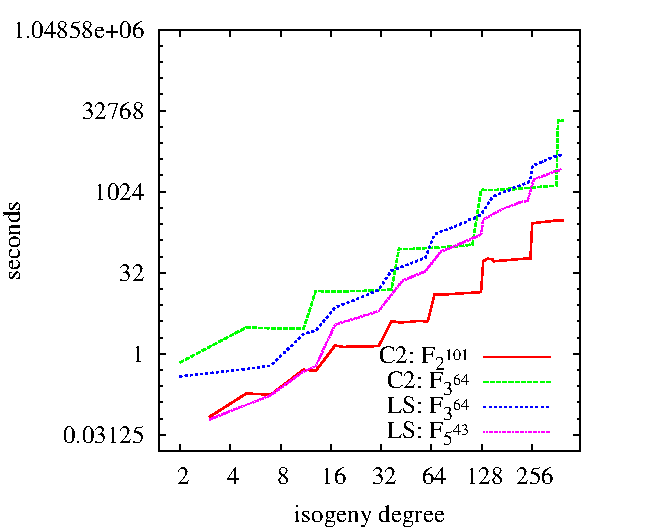
\includegraphics[height=0.5\textwidth]{../isogeny/C2-LS}
    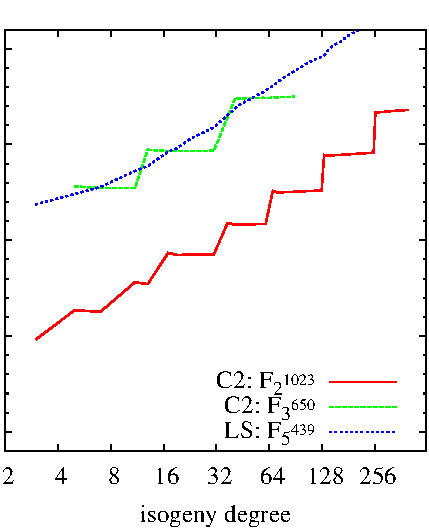
\includegraphics[height=0.5\textwidth]{../isogeny/C2-LS2}
    \caption{Comparative timings for \cite{couveignes96} (C2) and
      \cite{lercier+sirvent08} (LS) over various curves. Plot in
      logarithmic scale.}
  \label{fig:comp}
\end{figure}
\end{frame}

\begin{frame}
  \frametitle{Isogenies of unknown degree}
  \large

  \begin{itemize}
  \item This variant of \cite{couveignes96} is at the moment the
    fastest (both in theory and in practice) algorithm for this
    task.
  \item We tested two curves over $\F_{2^{161}}$, isogenous of
    unknown degree, taken from \cite{teske06}: proven in 694
    cpu-hours that no isogeny of degree less then $2^{13}$ exists.
  \end{itemize}
\end{frame}

%%
%%

\section{Artin-Schreier towers}

\begin{frame}
  \frametitle{The field of definition of $E[p^k]$}
  
  \begin{columns}
    \begin{column}{0.3\textwidth}
      \large\[\xymatrix@C=20pt{
        *[r]{\U_k} \ar@{-}[d]^p & E[p^k] \ar@{-->}[l]\\
        *[r]{\U_{k-1}} \ar@{--}[dd] & E[p^{k-1}] \ar@{-->}[l]\\
        \\
        *[r]{\U_2} \ar@{-}[d]^p & E[p^2] \ar@{-->}[l]\\
        *[r]{\U_1} \ar@{-}[d] & E[p] \ar@{-->}[l]\\
        *[r]{\F_q}
      }\]
    \end{column}
    \begin{column}{0.65\textwidth}
      \begin{center}
        \begin{tikzpicture}[node distance=4em]
          \node(C){$C$}; 
          \node(E)[below of=C]{$E$};
          \node(sqE)[left of=E]{$\widetilde{E}$};
          \scriptsize
          \textcolor<4>{red}{\path[->] (E) edge node[auto,swap]{$\simeq$} (C);}
          \textcolor<3>{red}{\path[->] (C) edge[bend right] (sqE);}
          \textcolor<2>{red}{\path[->] (sqE) edge[bend left] node[auto]{$\frobisog$} (E);}
          \path[->] (E) edge[dashed, bend left]  node[auto]{$V$} (sqE);
        \end{tikzpicture}
      \end{center}
      \begin{block}{$p$-descent (\cite{voloch90})}
        If $\;P_i=(x_i,y_i)\;$ generates $\;E[p^i]$, the solution to
        \begin{equation*}
          \begin{cases}
            \alert<3>{Z^p - Z} &\alert<3>{- \frac{\sqrt[p]{y_i\beta_E(x_i)}}{\sqrt[p-1]{H_E}}}\\
            \alert<2>{X^p} &\alert<2>{- x_i}\\
            \alert<2>{Y^p} &\alert<2>{- y_i}
          \end{cases}
        \end{equation*}
        generates $\;C[p^{i+1}]$.\\
        \alert<4>{Then apply the isomorphism $\;C\isom E$}.
      \end{block}
    \end{column}
  \end{columns}
\end{frame}

%%

\begin{frame}
  \frametitle{Artin-Schreier towers}

  \begin{columns}
    \begin{column}{0.3\textwidth}
      \Large\[\xymatrix{
        *+[r]{\U_k = \frac{\U_{k-1}[X_k]}{X_k^p-X_k-\alpha_{k-1}}}\ar@{-}[d]^p\\
        *+[r]{\U_{k-1}} \ar@{--}[dd]\\
        \\
        *+[r]{\U_{1} = \frac{\U_0[X_1]}{X_1^p-X_1-\alpha_0}} \ar@{-}[d]^p\\
        *+[r]{\U_{0} = \F_q = \frac{\F_p[X_0]}{Q(X_0)}}
      }\]
    \end{column}
    \begin{column}{0.65\textwidth}
      \begin{block}{Artin-Schreier polynomials}
        Artin-Schreier polynomial: 
        \begin{center}
          \emph{\large$X^p - X - \alpha\qquad$} with $\alpha\in\K$
        \end{center}
      \end{block}
      
      \begin{block}{Proposition}
        $X^p-X-\alpha\;$ is either irreducible or split in $\;\K$.
      \end{block}

      \begin{block}{Artin-Schreier extensions}
        Defined by an irreducible Artin-Schreier polynomial
        \begin{center}
          \large\emph{$\LK = \K[X]/(X^p - X - \alpha$)}
        \end{center}
        \alert{ANY} separable extension of degree $p$ can be expressed
        this way.
      \end{block}
    \end{column}
  \end{columns}
\end{frame}

%%

\begin{frame}
  \frametitle{Arithmetic in towers of extensions}
  
  \begin{columns}
    \begin{column}{0.3\textwidth}
      \Large\[\xymatrix{
        *+[r]{\U_k = \frac{\U_{k-1}[X_k]}{X_k^p-X_k-\alpha_{k-1}}}\ar@{-}[d]^p\\
        *+[r]{\U_{k-1}} \ar@{--}[dd]\\
        \\
        *+[r]{\U_{1} = \frac{\U_0[X_1]}{X_1^p-X_1-\alpha_0}} \ar@{-}[d]^p\\
        *+[r]{\U_{0} = \F_q = \frac{\F_p[X_0]}{Q(X_0)}}
      }\]
    \end{column}
    \begin{column}{0.65\textwidth}
      \begin{block}{Multiplication}
        \vspace{-\baselineskip}
        \begin{align*}
          \Mult(\U_0) &= O\bigl(\Mult(d)\bigr)\\
          \Mult(\U_1) &= O\bigl(p^2\Mult(d)\bigr)\\
          \Mult(\U_2) &= O\bigl(p^4\Mult(d)\bigr)\\
          &\vdots\\
          \Mult(\U_k) &= O\bigl(p^{2k}\Mult(d)\bigr) \varsupsetneq \tildO(p^kd)
        \end{align*}
        
        Even using Karatsuba or FFT multiplication, $\tildO(p^kd)$
        can't be attained.
      \end{block}
      \vspace{-1.5mm}
      \begin{block}{Other operations}
        \begin{itemize}
        \item Exponentiation, Inversion, GCD, all depend upon $\;\Mult(\U_k)$,
        \item The canonical injection $\;\U_{i-1}\ra\U_i$ can be computed in $O(p^i)$.
        \end{itemize}
      \end{block}
    \end{column}
  \end{columns}
\end{frame}

%%

\begin{frame}
  \frametitle{One fast tower, many fast towers!}
  
  \begin{center}
    A Fast A-S tower

    \smallskip

    \large$\xymatrix{
      \only<2->{E[p^k]\ar@{-->}[r]} & \only<2->{\U_k \ar@{-}[d]\ar[r]}      & \LK_k \ar@{-}[d]      & \only<2->{\U_k' \ar@{-}[d]\ar[l]}& \only<2->{E'[p^k]\ar@{-->}[l]}\\
      &\only<2->{\U_{k-1} \ar@{--}[dd]\ar[r]} & \LK_{k-1} \ar@{--}[dd] & \only<2->{\U_{k-1}' \ar@{--}[dd]\ar[l]}\\
      \\
      &\only<2->{\U_1 \ar@{-}[dr]\ar[r]}     & \LK_1 \ar@{-}[d]      & \only<2->{\U_1' \ar@{-}[dl]\ar[l]}\\
      &                    &\LK_0
    }$
  \end{center}

  \uncover<2->{ \emph{Theorem (\cite{couveignes00}):} There exist an
    isomorphism algorithm that runs in \alert{$O(k^3\Mult(\LK_k))$}
    operations in $\LK_0$. (Remember that \alert{$\;k=\log_p\card{\LK_k}$})}
\end{frame}

%%

\begin{frame}
  \frametitle{A fast tower}

  \begin{tikzpicture}
    \begin{scope}
      \draw (0,0) node {\Large$\xymatrix{
          *+[r]{\LK_k = \frac{\LK_{k-1}[X_k]}{X_k^p-X_k-\alpha_{k-1}}}\ar@{-}[d]^p\\
          *+[r]{\LK_{k-1}} \ar@{--}[d]\\
          *+[r]{\LK_1 = \frac{\LK_0[X_1]}{X_1^p-X_1-\alpha_0}} \ar@{-}[d]^p\\
          *+[r]{\LK_0 = \F_q = \frac{\F_p[X_0]}{Q(X_0)}} \ar@{-}[d]^d\\
          *+[r]{\F_p}
        }$};
    \end{scope}

    \begin{scope}[xshift=1.8cm]
      \draw (2,1) node {\parbox{3.3cm}{\emph{Idea:} Convert to a univariate basis \alert{over $\F_p$}}};
      \uncover<2->{\draw[<->] (0.4,0) -- (4,0);}
    \end{scope}
      
    \begin{uncoverenv}<2->
      \begin{scope}[xshift=8cm]
        \draw (0,0) node {\Large$\xymatrix{
            *+[r]{\LK_k = \frac{\F_p[Y_k]}{Q_k(Y_k)}}\ar@{-}[d]^p\\
            *+[r]{\LK_{k-1}} \ar@{--}[d]\\
            *+[r]{\LK_1 = \frac{\F_p[Y_1]}{Q_1(Y_1)}} \ar@{-}[d]^p\\
            *+[r]{\LK_0 = \F_q = \frac{\F_p[X_0]}{Q(X_0)}} \ar@{-}[d]^d\\
            *+[r]{\F_p}
          }$};
      \end{scope}
    \end{uncoverenv}
  \end{tikzpicture}
\end{frame}

%% 

\begin{frame}
  \frametitle{A fast tower: the multivariate side}

  \vspace{-2mm}

  \begin{columns}
    \begin{column}{0.3\textwidth}
      \Large$\xymatrix{
          *+[r]{\LK_k = \frac{\LK_{k-1}[X_k]}{X_k^p-X_k-x_{k-1}^{2p-1}}}\ar@{-}[d]^p\\
          *+[r]{\LK_{k-1}} \ar@{--}[d]\\
          *+[r]{\LK_1 = \frac{\LK_0[X_1]}{X_1^p-X_1-x_0}} \ar@{-}[d]^p\\
          *+[r]{\LK_0 = \F_q = \frac{\F_p[X_0]}{Q(X_0)}} \ar@{-}[d]^d\\
          *+[r]{\F_p}
        }$
    \end{column}
    \begin{column}{0.65\textwidth}
      \begin{block}{Our construction (inspired by \cite{cantor89})}
        \begin{equation*}
          \left\{
            \begin{array}{r@{}c@{}c@{}c@{}c@{}r@{}c@{}l}
              X^p_i & -X_i & -X_{i-1}^{2p-1}\\
              &&\vdots\\
              &&&X_2^p & -X_2 & -X_1^{2p-1}\\
              &&&&&X_1^p & -X_1 & -X_0\\
              &&&&&&&Q(X_0)
            \end{array}
          \right.
        \end{equation*}


        \emph{Theorem:} Let $\;x_i\;$ be the class of $\;X_i\;$ in
        $\;\LK_i\;$ (and thus in $\;\LK_{i+1},\ldots$).  If
        $\;\Tr_{\LK_0/\F_p}(x_0) \ne 0$, each line contains an
        irreducible polynomial and \alert{$x_i$ generates $\LK_i$ over
          $\F_p$.}
      \end{block}
    \end{column}
  \end{columns}
\end{frame}

%%

\begin{frame}
  \frametitle{A fast tower: the univariate side}

  \vspace{-2mm}

  \begin{columns}
    \begin{column}{0.3\textwidth}
      \Large$\xymatrix{
        *+[r]{\LK_k = \frac{\F_p[Y_k]}{Q_k(Y_k)}}\ar@{-}[d]^p\\
        *+[r]{\LK_{k-1}} \ar@{--}[d]\\
        *+[r]{\LK_1 = \frac{\F_p[Y_1]}{Q_1(Y_1)}} \ar@{-}[d]^p\\
        *+[r]{\LK_0 = \F_q = \frac{\F_p[X_0]}{Q(X_0)}} \ar@{-}[d]^d\\
        *+[r]{\F_p}
      }$    
    \end{column}
    \begin{column}{0.65\textwidth}
      \begin{block}{Univariate representation}
        The minimal polynomials $\;Q_i\;$ of $\;x_i\;$ over $\;\F_p\;$
        can be computed as follows.
        \begin{itemize}
        \item $Q_0 = Q$;
        \item $Q_1 = Q_0(Z^p-Z)$.
        \end{itemize}
        Let $\;\omega\;$ be a $\;(2p-1)$-th root of unity,
        \begin{itemize}
        \item $q_{i+1}(Z^{2p-1}) = \prod_{j=0}^{2p-2}Q_i(\omega^jZ)$,
        \item $Q_{i+1} = q_{i+1}(Z^p-Z)$.
        \end{itemize}
      \end{block}
    \end{column}
  \end{columns}
\end{frame}

%%

\begin{frame}
  \frametitle{A fast tower: change of basis}

  \vspace{-2mm}

  \begin{columns}
    \begin{column}{0.1\textwidth}
      \Large\[\xymatrix{
        \LK_k \ar@{-}[d]^p\\
        \LK_{k-1} \ar@{--}[dd]\\
        \\
        \LK_1 \ar@{-}[d]^p\\
        \LK_0 \ar@{-}[d]^d\\
        \F_p
      }\]
    \end{column}
    \begin{column}{0.85\textwidth}

      \begin{block}{Two bases to represent $\LK_k$}
        \begin{itemize}
        \item Univariate: \hfill\emph{$\LK_k=\F_p[Y_k]/Q_k(Y_k)$}\hfill
        \item Multivariate: \hfill\emph{$\LK_k=\F_p[X_0,X_1,\ldots,X_k]/(Q,\ldots)$}\hfill
        \end{itemize}
        \alert{A fast change of basis is the key to fast arithmetic:}
        \begin{itemize}
        \item Multiplication is faster in \emph{univariate};
        \item Field embeddings are faster in \emph{multivariate}.
        \end{itemize}
      \end{block}

      \begin{block}{Change of basis}
        \emph{Univariate $\ra$ multivariate}
        \begin{itemize}
        \item Recursively split input in $p$ slices, recombine by
          Horner's rule;
        \item Simple and fast: \emph{$\;O(\Mult(\ell) + \ell\log^2\ell)$}
        \end{itemize}
        
        \emph{Multivariate $\ra$ univariate}
        \begin{itemize}
        \item Trace formulas + duality + transposed algorithms;
        \item Same complexity: \emph{$\;O(\Mult(\ell) + \ell\log^2\ell)$}
        \end{itemize}
      \end{block}
    \end{column}
  \end{columns}
\end{frame}

\begin{frame}
  \frametitle{Example: univariate $\ra$ multivariate}
  
  \begin{center}
    \large\emph{$\F_{3^9} \;=\; \F_3[X_1,X_2]/I \;=\; \F_3[Y_2]/Q_2(Y_2)$}
  \end{center}

  \begin{gather*}
    I = 
    \begin{cases}
      &\alert<3>{X_2^3 - X_2 - X_1^5}\text{,}\\
      &X_1^3 - X_1 - 1\text{,}
    \end{cases}
    \\
    Q_2(Z) = Z^9 + Z^6 + Z^4 + Z^2 - Z - 1\text{,} \qquad Q_2(x_2) = 0\text{,}
  \end{gather*}

  \bigskip

  Let $a$ be given on the univariate basis:

  \smallskip

  \mbox{$a = \underbrace{X_2^8 + X_2^7 + X_2^6} + \underbrace{X_2^5} +
    \underbrace{X_2} = \uncover<2->{\alert<3>{X_2^6}(\underbrace{X_2^2
        + X_2 + 1}_{a_2}) + \alert<3>{X_2^3}(\underbrace{X_2^2}_{a_1})
      + (\underbrace{X_2}_{a_0})}$}
  
  \bigskip
  \uncover<3->{Then, $a = \left(\alert<3>{X_2 + X_1^5}\right)\left((\alert<3>{X_2 + X_1^5})a_2
      + a_1\right) + a_0\uncover<4->{\alert{\mod (X_2^3 - X_2 - X_1^5)=}}$}

  \bigskip

  \uncover<4->{\alert{$(X_1^2 - X_1 - 1)X_2^2 + (X_1 - 1)X_2 - X_1^2 - X_1 -1$}}
\end{frame}

%%

\begin{frame}
  \frametitle{Multivariate $\ra$ univariate}


  \begin{block}{Trace formulas (\cite{rouiller99})}
      \[
      a(Z) = \frac{A(Z)}{Q_k'(Z)}\bmod Q_k(Z)
      \qquad\text{where}\qquad
      A(T) = Q_k(T)\alert<2>{\sum_{i\ge 0}\frac{\Tr ax_k^i}{T^{i+1}}}
      \text{.}\]
    \begin{itemize}
    \item Compute the \textit{trace form} $\;\Tr\;$,
    \item compute the form $\;a\cdot\Tr : x\mapsto \Tr ax$,
    \item \alert<2>{compute $\;\sum_{i\ge 0}\frac{a\cdot\Tr x_k^i}{T^{i+1}}$},
    \item deduce $\;a(Z)$.
    \end{itemize}
  \end{block}

  \emph{Example:} Let $a = x_1$, then
  \begin{align*}
    A(T) &= Q_k(T) \left(\alert<2>{T^{-6} - T^{-8} - T^{-9} + O(T^{-10})}\right) = T^3 - T\text{,}\\
    a &= \frac{x_2^3 - x_2}{x_2^3 - x_2 - 1} = x_2^6 +
    x_2^4 - x_2^3 + x_2^2 + x_2 + 1\text{.}
  \end{align*}
\end{frame}

%%

\begin{frame}
  \frametitle{Duality (\cite{shoup95,shoup99,bostan+salvy+schost03})}

  \vspace{-6mm}

  \begin{columns}[b]
    \begin{column}{0.4\textwidth}
      \begin{center}
        \textbf{Polynomial evaluation}$:k[Z]\ra\K/k$
        \[g\mapsto g(\sigma)\]
      \end{center}
    \end{column}
    \begin{column}{0.6\textwidth}
      \begin{center}
        \textbf{Power projection}$:(\K/k)^\ast\ra k[T]^\ast \simeq k[[1/T]]$
        \[\ell \mapsto \sum_{i>0} \frac{\ell(\sigma^i)}{T^i}\]
      \end{center}
    \end{column}
  \end{columns}

  \begin{block}{Univariate $\ra$ multivariate $=$ Polynomial evaluation}
    If $Z \mapsto x_k\;$ (with $x_k\in\U_k$ written on the
    multivariate basis):
    \[a(Z) = a_dZ^d + \cdots + a_1Z + a_0 \quad\mapsto\quad a_dx_k^d + \cdots + a_1x_k + a_0 =a(x_k) = a\text{.}\]
  \end{block}

  \begin{block}{Transposed univariate $\ra$ multivariate $=$ Power projection}
    \begin{align*}
      \Tr &\quad\mapsto\quad \sum_{i\ge0}\frac{\Tr x_k^i}{T^i}\text{,}\\
      a\cdot\Tr &\quad\mapsto\quad \sum_{i\ge0}\frac{\Tr ax_k^i}{T^i}\text{.}
    \end{align*}
  \end{block}
\end{frame}

%%

\begin{frame}
  \frametitle{The transposition principle}

  \large
  
  \begin{theorem}
    ``Let $\pspace$ be an arbitrary set. To any $R$-algebraic
    algorithm $A$ computing a family of linear functions $(f_p:M\ra
    N)_{p\in\pspace}$ corresponds an $R$-algebraic algorithm
    $\dual{A}$ computing the \emph{dual family}
    $(\dual{f}_p:\dual{N}\ra\dual{M})_{p\in\pspace}$. The algebraic
    time and space complexities of $\dual{A}$ are bounded by the time
    complexity of $A$.''
  \end{theorem}
  
\end{frame}

%%

\begin{frame}
  \frametitle{Change of basis}

  \begin{block}{Univariate $\ra$ multivariate}
    \begin{itemize}
    \item Recursively split input in $p$ slices, recombine by
      Horner's rule;
    \item Simple and fast: \emph{$\;O(\Mult(\ell) + \ell\log^2\ell)$}
    \end{itemize}
  \end{block}

  \vspace{-1mm}

  \begin{block}{Multivariate $\ra$ univariate\hfill\alert{$\;O(\Mult(\ell) + \ell\log^2\ell)$}}
    By \textit{trace formulas} (\cite{rouiller99}):
    \[
    a(Z) = \frac{A(Z)}{Q_k'(Z)}\bmod Q_k(Z)
    \qquad\text{where}\qquad
    A(T) = Q_k(T)\sum_{i\ge 0}\frac{\Tr ax_k^i}{T^{i+1}}
    \text{.}\]
    \vspace{-4mm}
    \begin{itemize}
    \item Compute the \textit{trace form} $\;\Tr\;$ and the form
      $\;a\cdot\Tr : x\mapsto \Tr ax$;
    \item compute $\;\sum_{i\ge 0}\frac{a\cdot\Tr x_k^i}{T^{i+1}}$
      \alert{using a transposed univariate $\ra$ multivariate};
    \item deduce $\;a(Z)$.
    \end{itemize}
  \end{block}
\end{frame}

%%
%%

\section{Implementations}

\begin{frame}
  \frametitle{Implementations}


  \begin{block}{Automatic transposition}
    \begin{itemize}
    \item Algorithms are hard to transpose, transposed algorithms are
      hard or impossible to understand;
    \item How to be confident that a transposed algorithm is well
      implemented if no one understands it?
    \item When proving programs with a proof assistant, why should we do
      the work twice?
    \end{itemize}

    \hfill\emph{\url{http://transalpyne.gforge.inria.fr/}}\hfill\strut

    A Python-like ad-hoc language for automatic transposition,
    compiled/interpreted in Python.
  \end{block}
  
  \begin{block}{Artin-Schreier towers and isogenies}
    \begin{itemize}
    \item \emph{FAAST} (Fast Arithmetic in Artin-Schreier towers):
      \texttt{C++} with NTL implementation released under GPL:

      \hfill\emph{\url{http://www.lix.polytechnique.fr/~defeo/FAAST/}}\hfill\strut
    \item With F.~Morain and É.~Schost, writing a \texttt{C++} library
      for isogenies over finite fields.
    \end{itemize}
  \end{block}
\end{frame}

%%

\section{Conclusion}

\begin{frame}
  \frametitle{Perspectives}

  \begin{block}{The future of \texttt{transalpyne}}
    \begin{itemize}
    \item Finish the implementation, add more output languages.
    \item Integration in a Computer Algebra System (Sage?
      Mathemagix?).
    \item Development in a dependently typed system (Coq? Agda?).
    \end{itemize}
  \end{block}

  \begin{block}{Perspectives on isogenies}
    \begin{itemize}
    \item All known algorithms to compute isogenies have suboptimal
      complexity $\Omega(\ell^2)$.
    \item Are there models, where algorithms \textit{à la} BMSS and
      \cite{lercier+sirvent08} may be faster?
    \item Couveignes' first isogeny algorithm (\cite{couveignes94}) is
      very similar to \cite{couveignes96} and may be modified in the
      same way. There is some hope that it may be faster in practice,
      because of the simpler arithmetic operations needed.
    \item Generalize Couveignes' algorithms to genus $2$?
    \end{itemize}
  \end{block}
\end{frame}
\end{document}


% Local Variables:
% mode:flyspell
% ispell-local-dictionary:"american"
% mode:TeX-PDF
% mode:reftex
% End:
%
% LocalWords:  Isogeny abelian isogenies hyperelliptic supersingular Frobenius
% LocalWords:  isogenous
